% Problem 5/1 solution
\noindent
\underline{Solution:}\\
\begin{enumerate}
\item We calculate the expectation value ($\hat{H}\psi_1 = E_1\psi_1$ and $\hat{H}\psi_2 = E_2\psi_2$):
\begin{eqnarray}
\nonumber
& & \left<\hat{H}\right> = \int\psi^*(x)\hat{H}\psi(x)dx\\
\nonumber
& & = \frac{1}{2}\int\left(\psi_1^*(x) + \psi_2^*(x)\right)\hat{H}\left(\psi_1(x) + \psi_2(x)\right)dx
\end{eqnarray}

\begin{eqnarray}
\nonumber
& & = \frac{1}{2}\int\left(\psi_1^*(x) + \psi_2^*(x)\right)\left(E_1\psi_1(x) + E_2\psi_2(x)\right)dx = \frac{1}{2}\left(E_1 + E_2\right)\\
\nonumber
& & = 2.5\textnormal{ eV}
\end{eqnarray}

\item For $a = 1$ both $\psi_1(x)$ (one maximum) and $\psi_2(x)$ (maximum and minimum) are shown below:

\begin{figure}[htp!]
\centering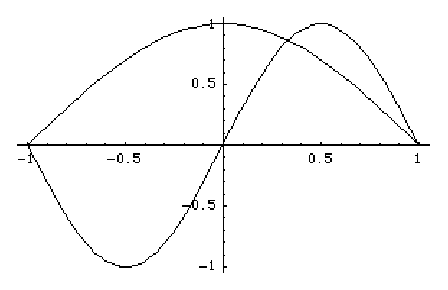
\includegraphics[scale=0.7]{wavefun1}
\end{figure}

The most probable values for position can be obtained from the squared wavefunctions:

\begin{figure}[htp!]
\centering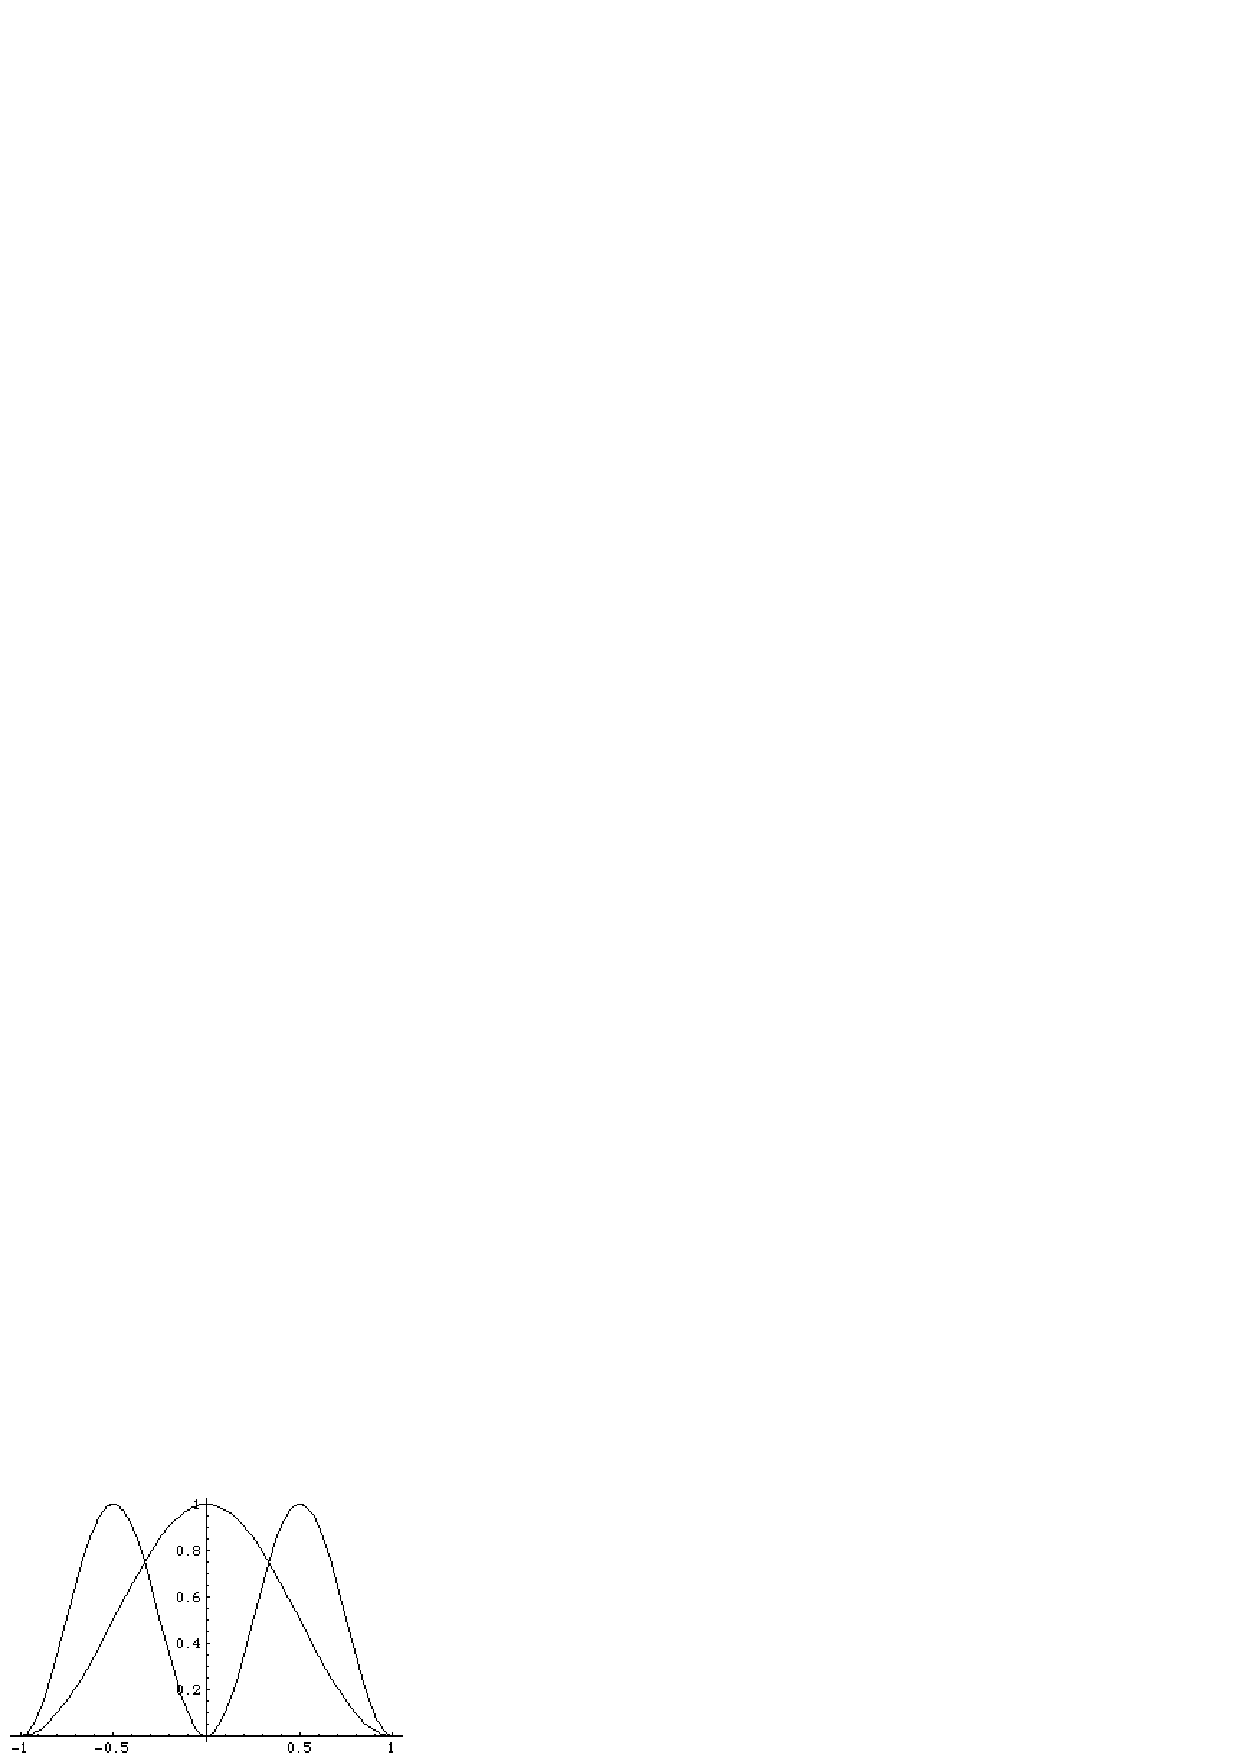
\includegraphics[scale=0.7]{wavefun2}
\end{figure}

$\psi_1$ has the maximum value at $r = 0$ whereas $\psi_2$ has two maxima at $\pm 0.5$. Note that on average both will give an outcome of $\left<\hat{r}\right> = 0$.

\item The most probable positions are given by the square of the wavefunction $\psi_0(x) = \left(2/L\right)^{1/2}\sin(3\pi x/L)$. The probability function is then $\left|\psi_0(x)\right|^2 \propto \sin^2(3\pi x/L)$. The extremum points for this function can be obtained by:
\begin{eqnarray}
\nonumber
& & \frac{d}{dx}\left(\sin^2(3\pi x/L)\right) = 0 \Rightarrow \sin(3\pi x/L)\cos(3\pi x/L) = 0\\
\nonumber
& & \Rightarrow \frac{3\pi x}{L} = n\pi\textnormal{ or }\frac{3\pi x}{L} = \left(n + \frac{1}{2}\right)\pi\\
\nonumber
& & \Rightarrow x = \frac{n}{3}L\textnormal{ or }x = \frac{n + 1/2}{3}L
\end{eqnarray}

Second derivatives can be used to identify the extrema:

$$\frac{d^2}{dx^2}\left(\sin^2(3\pi x/L)\right) \propto \cos^2\left(\frac{3\pi x}{L}\right) - \sin^2\left(\frac{3\pi x}{L}\right)$$

At $x = \frac{n}{3}L$ the values are positive which means that these correspond to (local) minima. For $x = \frac{n+1/2}{3}L$ the values are negative
and these points correspond to (local) maxima. For example, when $L = 2$ the probability function looks like:

\begin{figure}[htp!]
\centering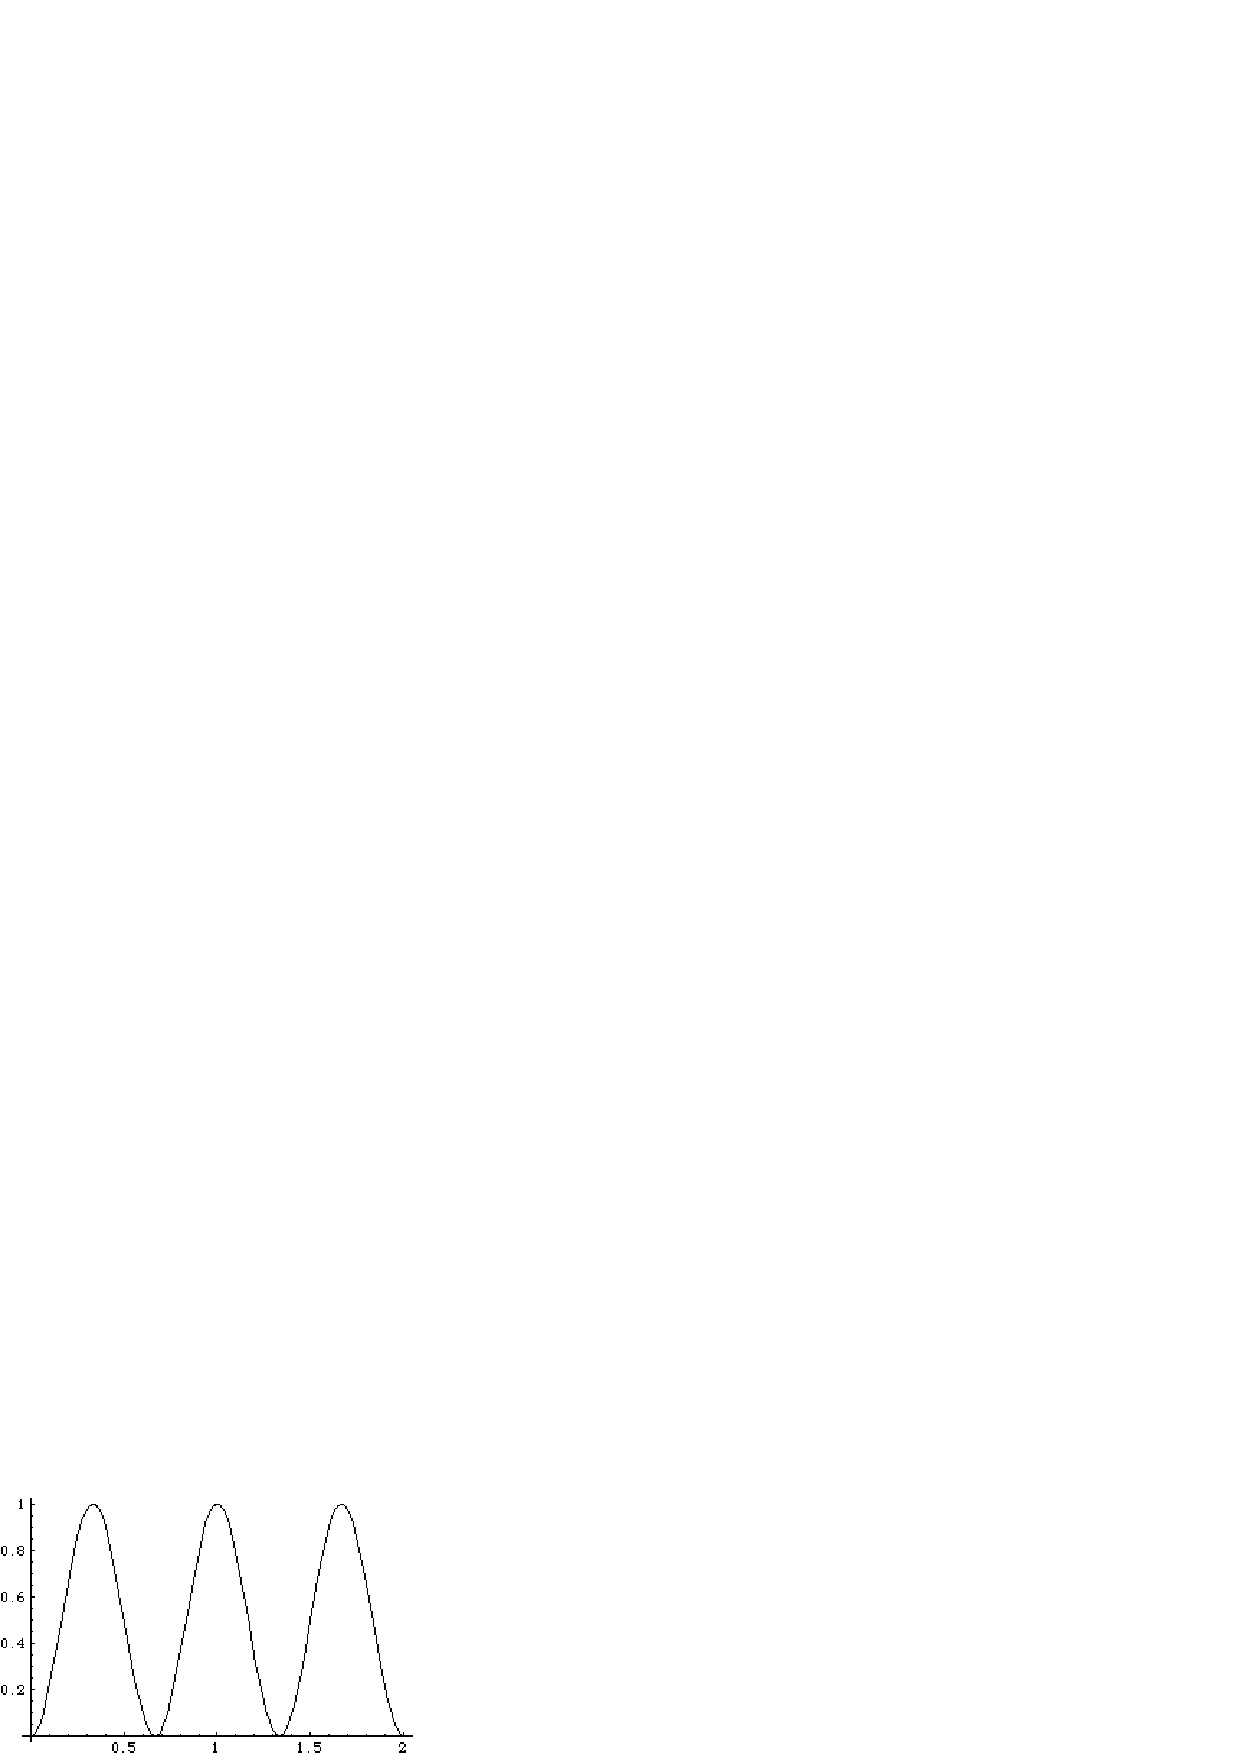
\includegraphics[scale=0.7]{wavefun3}
\end{figure}

\end{enumerate}

\hrule\vspace{0.5cm}
